% The spectrum figure: how many parameters the observable supports.
%
% Form: a sorted dot-and-stem plot on a log axis, not a bar chart. The data's
% job is to show WHERE a threshold falls in a sorted magnitude list, and the
% reference line at lambda = 1 is the whole point -- above it the data
% determines the direction, below it the prior does. A log axis is required
% because the values span four decades; a linear one would collapse fourteen of
% the fifteen onto the floor and hide the cliff, which is the finding.
%
% One series, so no legend: the title and the annotated threshold name
% everything. Colour is used only to separate the one supported direction from
% the fourteen that are not, and the separation is reinforced by the reference
% line and the labels, never by hue alone.
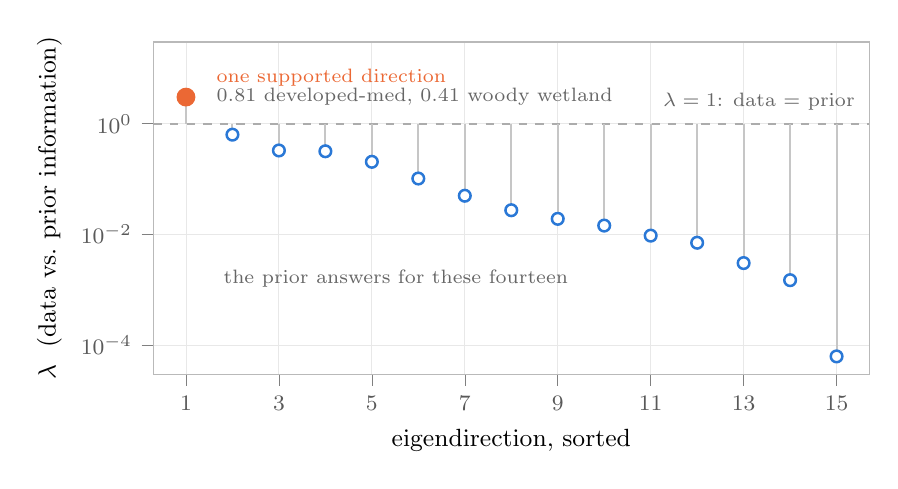
\begin{tikzpicture}
\begin{axis}[
  width=0.88\linewidth, height=5.8cm,
  xlabel={eigendirection, sorted},
  ylabel={$\lambda$ \ (data vs.\ prior information)},
  xmin=0.3, xmax=15.7,
  ymin=3e-5, ymax=30,
  ymode=log,
  xtick={1,3,5,7,9,11,13,15},
  tick align=outside, tick pos=left,
  axis line style={gray!55},
  tick label style={font=\footnotesize, color=black!65},
  label style={font=\small},
  grid=major, grid style={gray!18, line width=0.3pt},
  clip=false,
]

% the lambda = 1 threshold: data information equals prior information
\addplot[gray!65, line width=0.8pt, dashed, forget plot]
  coordinates {(0.3,1) (15.7,1)};
\node[font=\scriptsize, color=black!60, anchor=south east]
  at (axis cs:15.6,1.15) {$\lambda = 1$: data $=$ prior};

% stems
\addplot[ycomb, gray!45, line width=0.7pt, forget plot]
  coordinates {(1,3.033) (2,0.6353) (3,0.3292) (4,0.3183) (5,0.2055)
               (6,0.1025) (7,0.05008) (8,0.02742) (9,0.01917) (10,0.01448)
               (11,0.00953) (12,0.007093) (13,0.003043) (14,0.001495)
               (15,0.00006272)};

% the fourteen the prior determines
\addplot[only marks, mark=*, mark size=2.1pt,
         color={rgb,255:red,42;green,120;blue,214},
         mark options={fill=white, line width=0.9pt}, forget plot]
  coordinates {(2,0.6353) (3,0.3292) (4,0.3183) (5,0.2055)
               (6,0.1025) (7,0.05008) (8,0.02742) (9,0.01917) (10,0.01448)
               (11,0.00953) (12,0.007093) (13,0.003043) (14,0.001495)
               (15,0.00006272)};

% the one the data determines
\addplot[only marks, mark=*, mark size=3.2pt,
         color={rgb,255:red,235;green,104;blue,52},
         mark options={fill={rgb,255:red,235;green,104;blue,52}}, forget plot]
  coordinates {(1,3.033)};

\node[font=\scriptsize, color={rgb,255:red,235;green,104;blue,52},
      anchor=west, align=left]
  at (axis cs:1.45,4.6) {one supported direction\\[-1pt]
                         \textcolor{black!60}{$0.81$ developed-med, $0.41$ woody wetland}};
\node[font=\scriptsize, color=black!60, anchor=west, align=left]
  at (axis cs:1.6,0.0016) {the prior answers for these fourteen};
\end{axis}
\end{tikzpicture}
